\chapter{Resultados e Discussão}
\label{chap:resultados}

Neste capítulo, trazemos os achados e a análise dos mesmos utilizando a \acrlong{ARS} (\acrshort{ARS}) juntamente com o discurso dos entrevistados para aprofundar qualitativamente os achados e para fomentar a discussão.  As respostas foram fornecidas objetivando vislumbrar a caracterização e o funcionamento desta rede para pacientes hipertensos e diabéticos. 

\section{Análise da Rede Social: o enfermeiro ocupando espaços de destaque no sistema de saúde}

Analisar redes sociais permite vislumbrar as interações entre qualquer classe de indivíduos, partindo tanto de dados qualitativos quanto quantitativos. Segundo \cite{stanley1994social},  o uso de  análise de redes sociais possibilita coletar informações relevantes sobre a estrutura de um grupo, sendo possível, identificar as posições ocupadas pelos indivíduos, bem como identificar o cerne das relações criadas ao redor de cada um.

Como explicado anteriormente, os dados foram coletados no município de Icapuí-Ce, considerando a primeira entrevistada para seguir o processo. Tendo como foco a linha de cuidado de pessoas que tem hipertensão arterial e diabetes. 

Logicamente, uma infinidade de análises pode ser realizada considerando os dados coletados, o que pode ser inviável de abordar em um único trabalho. Portanto, um número limitado de atores, conexões e métricas foi utilizado, e a partir deles, foram feitas considerações sobre o comportamento geral da rede social de uma única enfermeira. 

A rede pesquisada não contempla todas as relações possíveis e existentes de cada pessoa entrevistada, mas somente um recorte viável de analisar. As notações consideradas no desenho do grafo estão reunidas nas tabelas \ref{graph-job} e \ref{graph-place}.

\begin{table}[htbp]
\centering
\caption{Significado dos rótulos dos atores da rede segundo suas profissões.}
\label{graph-job}
\begin{tabular}{|l|l|}
\hline
Notação  & Profissão               \\ \hline
E        & Enfermeiro(a)           \\ \hline
E{[}R{]} & Enfermeiro(a) Residente \\ \hline
F        & Farmacêutico(a)         \\ \hline
N        & Nutricionista           \\ \hline
N{[}R{]} & Nutricionista Residente \\ \hline
M        & Médico(a)               \\ \hline
A        & Outro                   \\ \hline
\end{tabular}
\end{table}

\begin{table}[htbp]
\centering
\caption{Significado dos rótulos dos atores da rede segundo as áreas de atuação.}
\label{graph-place}
\begin{tabular}{|l|l|}
\hline
Notação & Área de Atuação                       \\ \hline
{[}H{]} & Hospital                      \\ \hline
{[}S{]} & Secretaria de Saúde de Icapuí \\ \hline
{[}P{]} & Policlínica de Aracati        \\ \hline
        & Atenção Básica                \\ \hline
\end{tabular}
\end{table}

Além disso, a identificação dos atores segue a seguinte notação [Profissão][Identificador Único] [Área de Atuação], por exemplo, $E1 [R]$ (Enfermeiro(a) 01 Residente); $E2$ (Enfermeiro 02 Atenção básica) etc.

Como pode ser observado na Figura \ref{fig:grafos}, o grafo permite identificar vinte e seis (26) atores que fazem parte da rede, onde seis (6) pessoas foram entrevistadas, vinte (20) outras foram citadas, trinta (30) relações e nenhum laço.

\begin{figure}[htbp]
\centering
 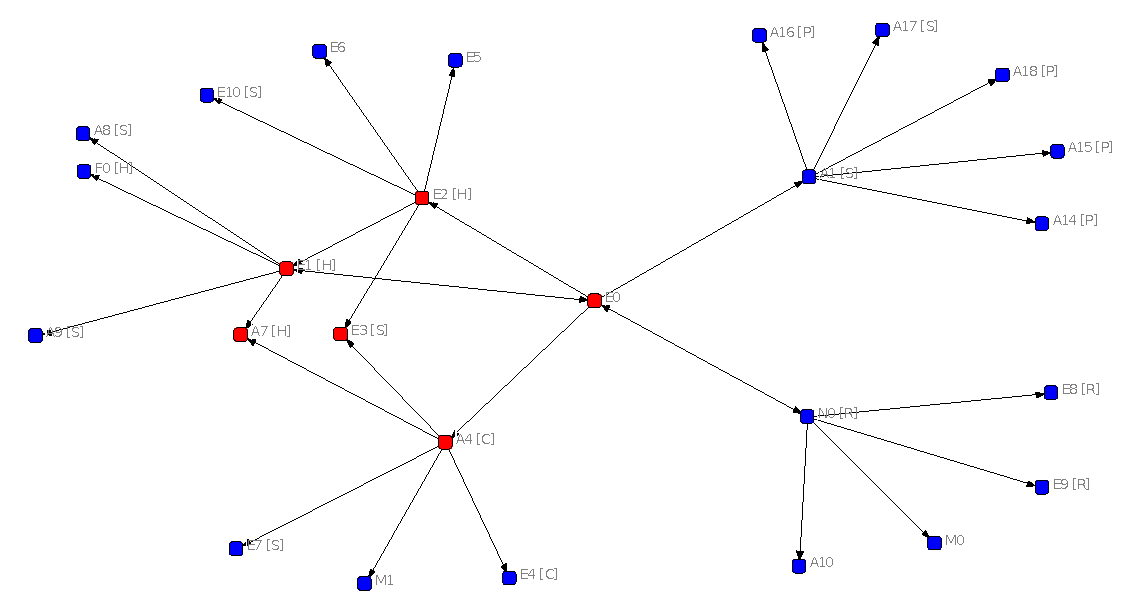
\includegraphics[width=.85\textwidth]{figuras/grafo-grupos.pdf}
 \caption{Representação da rede social utilizada neste trabalho.}
\label{fig:grafos}
\end{figure}

A primeira medida analisada da rede foi a densidade que é a relação entre o número de laços existentes e o número de laços possíveis. Tal métrica exibe a taxa de conectividade da rede. Neste trabalho, o valor de densidade encontrado foi de 4,61\% (baixa densidade) o que pode denotar a existência de alguma dificuldade na resolução de problemas em grupo.

Geralmente, nas circunstâncias onde existe baixa densidade, os atores não conseguem se identificar como participantes de um grupo maior e podem demonstrar certa dificuldade de relacionamento. Tal situação pode acarretar pouca cooperatividade entres os atores envolvidos, podendo até mesmo existir apatia na resolução de problemas, gerando conflitos. \cite{hanneman2001centralidad}.

Entretanto, devemos ressaltar que os atores identificados na rede localizam-se em diferentes espaços de trabalho, o que pode contribuir para uma comunicação mais limitada junto a outros possíveis atores. Além deste fato, as motivações de cada um dos entrevistados na denominação dos atores de suas redes, bem como o número de entrevistados devem ser levados em conta nesta análise como um fator interveniente na densidade. 

Outra medida importante é o grau de centralidade, ele indica o número de ligações que entram e que saem de um ator. Através dele são identificados os atores principais da rede. A tabela \ref{table-centralize-degree} exibe o grau de centralidade associado a cada ator.

\begin{table}[htbp]
\centering
\caption{Grau de centralização de cada ator.}
\label{table-centralize-degree}
\begin{tabular}{|l|l|l|l|l|}
\hline
Identificador & Grau de Saída & Grau de Entrada & Grau de Saída  & Grau de Entrada \\ 
	      &               &                 & Normalizada    & Normalizada \\ \hline
E0            & 5,000         & 2,000           & 0,200                     & 0,080                       \\ \hline
A1 {[}S{]}    & 5,000         & 1,000           & 0,200                     & 0,040                       \\ \hline
E1 {[}H{]}    & 5,000         & 2,000           & 0,200                     & 0,080                       \\ \hline
N0 {[}R{]}    & 5,000         & 1,000           & 0,200                     & 0,040                       \\ \hline
A4 {[}C{]}    & 5,000         & 1,000           & 0,200                     & 0,040                       \\ \hline
E2 {[}H{]}    & 5,000         & 1,000           & 0,200                     & 0,040                       \\ \hline
F0 {[}H{]}    & 0,000         & 1,000           & 0,000                     & 0,040                       \\ \hline
A7 {[}H{]}    & 0,000         & 2,000           & 0,000                     & 0,080                       \\ \hline
A8 {[}S{]}    & 0,000         & 1,000           & 0,000                     & 0,040                       \\ \hline
A9 {[}S{]}    & 0,000         & 1,000           & 0,000                     & 0,040                       \\ \hline
A10           & 0,000         & 1,000           & 0,000                     & 0,040                       \\ \hline
E9 {[}R{]}    & 0,000         & 1,000           & 0,000                     & 0,040                       \\ \hline
E8 {[}R{]}    & 0,000         & 1,000           & 0,000                     & 0,040                       \\ \hline
M0            & 0,000         & 1,000           & 0,000                     & 0,040                       \\ \hline
A14 {[}P{]}   & 0,000         & 1,000           & 0,000                     & 0,040                       \\ \hline
A15 {[}P{]}   & 0,000         & 1,000           & 0,000                     & 0,040                       \\ \hline
A16 {[}P{]}   & 0,000         & 1,000           & 0,000                     & 0,040                       \\ \hline
A17 {[}S{]}   & 0,000         & 1,000           & 0,000                     & 0,040                       \\ \hline
A18 {[}P{]}   & 0,000         & 1,000           & 0,000                     & 0,040                       \\ \hline
E10 {[}S{]}   & 0,000         & 1,000           & 0,000                     & 0,040                       \\ \hline
E3 {[}S{]}    & 0,000         & 2,000           & 0,000                     & 0,080                       \\ \hline
E6            & 0,000         & 1,000           & 0,000                     & 0,040                       \\ \hline
E5            & 0,000         & 1,000           & 0,000                     & 0,040                       \\ \hline
E4 {[}C{]}    & 0,000         & 1,000           & 0,000                     & 0,040                       \\ \hline
M1            & 0,000         & 1,000           & 0,000                     & 0,040                       \\ \hline
E7 {[}S{]}    & 0,000         & 1,000           & 0,000                     & 0,040                       \\ \hline
\end{tabular}
\end{table}

Através da tabela \ref{table-centralize-degree} identifica-se que os principais atores da rede são $E0$, $E1[H]$, $A7 [H]$ e  $E3[S]$ pois cada um possui Grau de Entrada Normalizada de 0,8 (mais requisitados).

$E0$ trata-se de uma enfermeira bastante conhecida no município, pois foi uma das primeiras enfermeiras a integrar a ESF quando esta foi implantada em Icapuí e ainda recebia a denominação de \acrlong{PSF} (\acrshort{PSF}). Está no quadro de funcionários do município como enfermeira desde o fim da graduação tendo passado também pelo Hospital Municipal, integrando a equipe assistencial. Em sua fala, $E0$ coloca que: 

\begin{citacao}
``Esse mesmo tempo, que quando eu me formei eu vim pra cá, e fiquei trabalhando aqui em Barreiras e mais em outra área, a gente conjugava duas unidade de saúde, quando iniciou a formação do PSF do município, então não tinha muito profissional na época, então a gente se dividia em duas equipes, com o passar do tempo que a gente foi... Eu to aqui só em Barreiras mesmo, esses vinte anos, mas eu sempre dividi até o ano passado dividi com outra unidade de saúde.''
\end{citacao}

Por esse longo período imersa na comunidade, inclusive em duas equipes, pela carência de profissionais na época, $E0$ teve a oportunidade de servir como referência a outros profissionais que adentraram no programa posteriormente. Seu período como plantonista no hospital, também proporcionou a ela o desenvolvimento de outras relações com outros profissionais, como $E1 [H]$ e $E2 [H]$.

$E1[H]$ é coordenador do serviço de enfermagem do hospital, além de enfermeiro plantonista. Adentrou no serviço de saúde do município exercendo o cargo de auxiliar de serviços gerais em 1990. A partir daí, fez cursos técnicos tanto na área de enfermagem como na área de análises clínicas, trabalhando na instituição tanto como técnico e auxiliar de enfermagem como técnico em radiologia por seis (6) anos. Graduou-se em Ciências Biológicas e em Enfermagem no ano de 2013. Exercendo atualmente as funções assistenciais e gerenciais na instituição.

$E1[H]$ cita $E0$ e é citado por esta, pois desenvolveram um vínculo devido ao período em que trabalharam juntos no hospital. $E1[H]$ chegou a se emocionar durante a entrevista ao falar de $E0$, denotando o desenvolvimento também de vínculo emocional. Ele relata:

\begin{citacao}
``Quer dizer é...em especial em termo de dedicação assim, eu gostaria até de destacar, a mesma pessoa que me indicou, porque é uma pessoa além de muito capacitada, muito sensível, muito humana, e... E a gente têm um perfil de profissional muito parecido. E ela, a $E0$, já faz parte da minha história também, né? ($E1[H]$).

Então é... Falando da enfermeira E0 novamente, eu tenho todo orgulho e satisfação, em dizer que à nossa aproximação se deu é...pela semelhança que a gente têm como profissional né, por esse feedback que existe, certo e...a gente têm um perfil de profissional muito parecido, eu já falei e to repetindo porque eu realmente to emocionado, ela acompanhou o meu trajeto, é...da minha profissão como eu falei anteriormente, desde o comecinho e me acompanha até hoje, e hoje a gente é colega de trabalho, e ela sempre me procura quando precisa, e isso faz um vínculo muito forte, que eu não quero que quebre nunca ($E1[H]$).''
\end{citacao}

Ao citar $A7[H]$, $E1[H]$ apontou a importância do contato baseado nas questões gerenciais, pois $A7[H]$, enquanto diretora administrativa do hospital, conseguia resolver as questões que $E1[H]$ não conseguia dar seguimento. Ao ser solicitado que relatasse uma situação na qual ele teve um problema que não conseguiu solucionar $E1[H]$ respondeu: ``A direção administrativa do hospital.($E1[H]$)''

$A7[H]$ também é apontada por $A4[C]$, técnica de enfermagem e atualmente recepcionista do CAPS do município, por ser apontada por ela como uma pessoa que resolve conflitos e facilita o acesso do usuário. $A4[C]$ conta: 

\begin{citacao}
``...e a terceira pessoa, a diretora do hospital, porque assim...sempre quando a gente tem um problema aqui no Caps, que a gente precisa de um atendimento médico mais o médico não tá aqui, aí eu passo pra enfermeira daqui de dentro, que ela é também coordenadora....e a diretora do hospital, porque às vezes o médico que ta de plantão, não conhece o trabalho do Caps, não conhece o paciente, se nega a fazer, então a diretora vai lá e aí ajeita tudo, e dá um jeito de contornar a situação né, paciente não ficar sem atendimento. ($A4[C]$)''
\end{citacao}


$E3[S]$ é enfermeiro e atualmente coordena a Atenção Básica. É citado por $A4[C]$ e por $E2[H]$. Estando em um cargo de gestão no município, entra em contato com diferentes profissionais e lida com diversas demandas. É apontado pelos entrevistados que o citaram como alguém sempre acessível e bem próximo a comunidade, conseguindo realizar pactuações e articulações. Seguem as falas que ilustram o fato:

\begin{citacao}
 ``...aí sempre a gente dar um jeitinho, por exemplo, vem um paciente, a família chega aqui diz assim, olha paciente tá lá em casa, surtou, né, teve uma crise muito grande, tá incontrolável, e aí? A gente vai lá no hospital, chama o $E3[S]$, o $E3[S]$ vai com o médico que tá de plantão no hospital, e aí a gente acaba trazendo o paciente, levando pro hospital e ele sendo atendido assim, nunca acontece dele não ter o atendimento, ($A4[C]$).
 
...às vezes acontece dum médico se recusar, mas aí a gente vai e comunica a secretaria de saúde, e aí $E3[S]$, ele é o coordenador, vai lá e conversa passa o caso pra ele, e aí tudo se resolve,($A4[C]$)

Hum, deixa eu ver. $E3[S]$ já foi? Porque $E3[S]$, é o coordenador da atenção básica...(risos) é porque ele está a par das situações...É...digamos, eu tenho que fazer uma busca ativa daquele paciente, quero saber como tá, ele já por ter toda essa rede de agilidade, conhece todo mundo, do agente de saúde de Redonda, ao agente de saúde de...esse povo que é a última unidade, que já é quase é  divisa com o Rio Grande, ele já têm mais esse conhecimento, aí já facilita. ($E2[H]$)''
\end{citacao}

Percebemos assim o importante papel que os profissionais de Enfermagem exercem na rede de atenção municipal, ocupando os diferentes espaços não apenas nos níveis de atenção, mas também em funções administrativas e de gestão de recursos. Nestas funções eles gerenciam recursos humanos, intermediando conflitos e mobilizando pessoas. O contato com a comunidade e a pertença ao território, facilitam as intermediações e a comunicação dos profissionais com a gestão e da comunidade com os serviços de saúde. 

O Grau de Proximidade denota a capacidade de um ator se ligar a todos os outros atores de uma rede, ou seja, quanto menor a distância entre um ator e outro, maior será seu grau de proximidade. 

Já o Grau de Intermediação mostra a capacidade que um ator possui de intermediar a comunicação entre pares de atores da rede. Sua importância se dá, pois, através de atores que possuem alto grau de intermediação que as informações são propagadas para diversos outros atores. 

A tabela \ref{closeness-betweeness-degree} lista o Grau de Proximidade e Intermediação dos atores.

\begin{table}[htbp]
\centering
\caption{Grau de Proximidade e Intermediação dos Nós.}
\label{closeness-betweeness-degree}
\begin{tabular}{|l|l|l|}
\hline
Identificador & Grau de Proximidade & Grau de Intermediação \\ \hline
E0            & 55.556              & 66.667                \\ \hline
A1 {[}S{]}    & 42.373              & 36.667                \\ \hline
E1 {[}H{]}    & 44.643              & 26.333                \\ \hline
N0 {[}R{]}    & 40.984              & 30.000                \\ \hline
A4 {[}C{]}    & 42.373              & 27.333                \\ \hline
E2 {[}H{]}    & 44.643              & 26.333                \\ \hline
F0 {[}H{]}    & 31.250              & 0.000                 \\ \hline
A7 {[}H{]}    & 35.211              & 2.667                 \\ \hline
A8 {[}S{]}    & 31.250              & 0.000                 \\ \hline
A9 {[}S{]}    & 31.250              & 0.000                 \\ \hline
A10           & 29.412              & 0.000                 \\ \hline
E9 {[}R{]}    & 29.412              & 0.000                 \\ \hline
E8 {[}R{]}    & 29.412              & 0.000                 \\ \hline
M0            & 29.412              & 0.000                 \\ \hline
A14 {[}P{]}   & 30.120              & 0.000                 \\ \hline
A15 {[}P{]}   & 30.120              & 0.000                 \\ \hline
A16 {[}P{]}   & 30.120              & 0.000                 \\ \hline
A17 {[}S{]}   & 30.120              & 0.000                 \\ \hline
A18 {[}P{]}   & 30.120              & 0.000                 \\ \hline
E10 {[}S{]}   & 31.250              & 0.000                 \\ \hline
E3 {[}S{]}    & 35.211              & 2.667                 \\ \hline
E6            & 31.250              & 0.000                 \\ \hline
E5            & 31.250              & 0.000                 \\ \hline
E4 {[}C{]}    & 30.120              & 0.000                 \\ \hline
M1            & 30.120              & 0.000                 \\ \hline
E7 {[}S{]}    & 30.120              & 0.000                 \\ \hline
\end{tabular}
\end{table}

A partir da tabela \ref{closeness-betweeness-degree} observa-se que os atores $E0$, $A1 [S]$, $E1 [H]$, $N0 [R]$, $A4 [C]$ e $E2 [H]$ possuem os maiores Graus de Proximidade e os atores $E0$, $A1 [S]$ e $N0 [R]$ possuem maiores Graus de Intermediação.

Nesta análise $E0$ possui maior grau de intermediação pois a rede foi construída a partir dela. Mas destaca-se a mesma medida de $A1[S]$. $A1[S]$ é responsável pela distribuição de um grande número de informações na rede. Ela possibilita o acesso a outros profissionais e serviços contactando atores de difícil acesso aos demais atores da rede, uma vez que encontra-se na Central de Marcação de Consultas do município, realizando o contato da rede municipal de Icapuí com a rede de Aracati através da policlínica.

Com as análises do grafo formado e as falas dos entrevistados, temos uma visão da importância do enfermeiro na rede e de outros profissionais da enfermagem que adentraram no serviço exercendo diferentes funções, desempenhando a comunicação  em diferentes espaços de trabalho.

Devemos atentar também para a importância da Residência Multiprofissional no município, uma vez que alguns profissionais residentes foram citados. $E0$ em sua fala coloca:

\begin{citacao}
``A gente na verdade se articula muito por conta do pessoal da residência a gente consegue resolver muita coisa, é mais a questão nutricional né, que muitas vezes a gente tem a questão dos hipertensos, diabéticos que dão trabalho em relação á hábito alimentar, a fisioterapeuta é mais a questão de prevenção, né nem de tratamento né, é mais de prevenção, orientação, de orientar essa questão da caminhada, dos exercícios, fortalecer. É mais isso. Mas de acompanhamento de tratamento é muito pouco.($E0$)''
\end{citacao}

Quando questionada a respeito de como era antes da Residência no município, E0 responde:

\begin{citacao}
``Mulher a gente encaminhava pra fisioterapia aqui, e a nutricionista a gente encaminhava pra Aracati. Era mais difícil né, pela questão do poder aquisitivo pra ir pra lá, e as vezes a pessoa vinha pra cá pela questão da proximidade. Mas as vezes nem quer aderir, quem quer que vá fazer adesão é a gente né, com acompanhamento da nutricionista. Aí pra ir pra Aracati, fica mais difícil, aqui se torna mais fácil. ($E0$)''
\end{citacao}

Percebemos aqui o impacto que a Residência Multiprofissional exerce na continuidade do cuidado e no fácil acesso a esses serviços. \cite{maia2013atuaccao} coloca o potencial gerado da experiência de interação entre os diversos saberes:

Essas trocas entre diferentes saberes geram uma nova configuração interna, que, se ouvida e entendida, cria a possibilidade de atitudes interdisciplinares. Isso quer dizer que a atitude inter não se dá porque duas ou mais profissões vão habitar o mesmo espaço, mas porque se produz um ambiente no qual os profissionais interagem, se comunicam, trocam e unem informações e conhecimentos.

A comunicação aparece bem vinculada aos enfermeiros e aos demais profissionais da enfermagem no grafo, e apesar de outros profissionais participarem da rede e serem citados, o desenho da rede aponta parauma necessidade de envolvimento de outros trabalhadores da saúde no processo.